\documentclass[10pt]{report}
\usepackage{scribe,graphicx,graphics}
\usepackage{amsmath}
\usepackage{amssymb}
\usepackage{listings}
\usepackage{color} %red, green, blue, yellow, cyan, magenta, black, white
\usepackage{caption}
\usepackage{subcaption}
\usepackage{eucal}
\usepackage{enumitem}
\usepackage{pythonhighlight}
\usepackage{url}
% \UseRawInputEncoding
\definecolor{mygreen}{RGB}{28,172,0} % color values Red, Green, Blue
\definecolor{mylilas}{RGB}{170,55,241}
% \input{../Output/inputs.tex}



\newcommand{\Op}{\mathcal{O}}
\newcommand{\argmax}{\operatornamewithlimits{argmax}}
\newcommand{\Reals}{\mathbb{R}}
\newcommand{\Naturals}{\mathbb{N}}
\course{ARE 212 - Part II}
\coursetitle{Econometrics}
\semester{Spring 2023}
\lecturer{} % Due Date: {\bf Mon, Oct 3 2016}}
\lecturetitle{1}

\lecturedate{}

% Insert your name here!
\scribe{Student Name: Bora Ozaltun, Sarah O'Brien, Scott Kjorlien, Garrison Schlauch}



\begin{document}
\maketitle

\section*{2. Exercises}
\subsection*{Part (1)}
Lets first remember the theorem:


\noindent ---
\begin{theorem}
    Let X take values in $E \subseteq \Reals^k$ be a $k \times 1$ absolutely continuous random vector with a probability density function $f_X(x)$. Let $g: E \rightarrow\Reals^k$ be a one-to-one, continuously differentiable function. Let $E_0$ be an open subset of $E$ such that $P(X \in E_0)=1$ and such that the Jacobian of g is non-zero on $E_0$.

    Then the $k \times 1$ random vector $Y=g(X)$ is absolutely continuous with probability density function given by:
    \[f_Y(y) = f_X(g^{-1}(y)) |\frac{\partial g^{-1}(y)}{\partial y}| \; \; \text{for } \; y \in g(E_0)\equiv Y_0\]
\end{theorem}
---
\;


For this question we are given that (x, y) are independent and continuously distributed random variables with densities $f_x, f_y$. Setting $z = x +y$, we are asked to write down a formula for $f_z$. Lets set up the problem so that we can use the theorem given above:

\begin{itemize}
    \item Since (x, y) are independent, $f_{(x, y)} = f_x f_y$.
    \item Define a function $g:E \rightarrow \Reals^2$ where $E \subseteq \Reals^2$ such that $ \begin{bmatrix}
        z\\
        k    
        \end{bmatrix} = g(x,y) = \begin{bmatrix}
    x + y\\
    y    
    \end{bmatrix}$. 
    \item Define the support of $(x, y)$ to be to be $E = \begin{pmatrix} E_1 \\ E_2 \end{pmatrix} \subseteq \Reals^2$. Further, define $E_0 \subseteq E$ to be the open subset of $E$  such that $P((x, y) \in E_0)=1$ and such that the Jacobian of g is non-zero on $E_0$. Finally, define $g(E_0) = \begin{pmatrix} A_0 \\ E_{0,2} \end{pmatrix}$, where $E_{0,1}$ might not be the same as $A_0$.
\end{itemize}

\noindent Now we can get the inverse of $g$ to be $g^{-1}(z, k) =  \begin{bmatrix}
    z - k\\
    k    
    \end{bmatrix}$. The Jacobian of $g^{-1}(z, k)$ can then be calculated as:
    \[\frac{\partial g^{-1}(z, k)}{\partial (z, k)} = \begin{bmatrix}
        1 & -1 \\
        0 & 1 \\
    \end{bmatrix}\]
    \noindent meaning the determinant is $|\frac{\partial g^{-1}(z, k)}{\partial (z, k)} | = 1$. By the Theorem above, we can finally calculate the density of $(z,k)$:
\[f_{(z, k)}(z, k) = f_{(x, y)}(z-k, k) = f_{x}(z - k) f_{y} (k)\; \; k \in E_{2,0} \; Z \in A_0\]
\noindent which finally leads us to the dis distribution of $z$ by integrating out $k$ (which is just $y$):
\[f_z(z) = \int_{A_0} f_{x}(z - k) f_{y} (k) dk\].

\subsection*{Part 2}
We are given that $s$ is a discrete random variable and $x$ is a continous random variable. Assuming that s and x are independent, we will show that the convolution has a continous cdf. Let $m = s + x$, the random variable that is a result of the convolution. So we can get the cdf to be:

\[P(m \leq a) = P(s + x \leq a) = \sum_{i \in supp(s)} P(s + x \leq a | s=i) P(s=i) = \sum_{i \in supp(s)} P(x \leq a-i) P(s=i)\]

\noindent Notice that $P(x \leq a-i)$ is the probability that the random variable $x$ is less than $a-i$. Since $x$ is a continuous random variable, its cdf will be continous as well. The weighted sum of continuous functions is also continuous, meaning that $P(m\leq a)$ must be continuous. This proves that the cdf is continuous.

Note that this doesn't guarantee continuity or even existence of the pdf of $z$. We would further need to assume that the pdf of $x$ exists and is continuous to guarantee that the pdf of $m$ is continuous. This requires additional assumptions as not all continuous random variables have pdfs and not all continuous random variables that do have pdfs have continuous pdfs.

Because of this last point, the code provided in class is a bit misleading. Even though we will get a continuous cdf as a result of the convolution, we don't have any guarantees that we will get a continuous pdf. The figure at the end of the notebook plots the pdf, which is a bit misleading since we don't know if the pdf exists or is even continuous. We can however plot the cdf and it will be continuous for all convolutions of discrete and continuous random variables.

\subsection*{Part 3}
We are given an $m \times n$ matrix A such that A is a matrix of zeros. For a generalized inverse $A^-$ of A, we need the following property to hold: $A A^- A = A$. Notice that for any finite matrix $B$ which is of size $nxm$, $A B = 0$ since A is a matrix of zeros. Then we can say that $A B A =0$. So any finite matrix is a generalized inverse of a matrix of zeros. 

\subsection*{Part 4}
The question asks us to suggest a notation for ``Why'' and ``Ex'' under different circumstances. In class, we are offered a set of notations, below we will suggest another set of notations:

\begin{enumerate}[label=(\alph*)]
    \item $Why=Y$ and $Ex=\boldsymbol{X}=(X_1, X_2, \ldots, X_n)$.
    \item $Why=y$ and $Ex=\boldsymbol{x} = (x_1, x_2, \ldots, x_k)$
    \item $Why=\boldsymbol{y}$ and $Ex=\boldsymbol{x^n} = (\boldsymbol{x_1},\boldsymbol{x_2}, \ldots, \boldsymbol{x_n})$
\end{enumerate}

\subsection*{Part 5}
\begin{enumerate}[label=(\alph*)]
    \item Note, since $r=0$ in the case where $A$ is a matrix of zeros, we don't have any guarantees that $A^{+}$ is unique. As we discussed in Part 3, there are many candidates that will satisfy the general inverse. This is also the case for the Moore-Penrose inverse. One such matrix that fits the criterias of the Moore-Penrose inverse is a matrix of zeros of dimension $n \times m$.
    \item Let X be $m \times n$. If $X$ has full column rank then $rank(X)=r=n\leq m$. Notice that in this case, a full rank factorization of $X$ is $L=X$, a $m\times n$ matrix, and $R = I_n$, a $n\times n$ matrix. L is full column rank by definition and R is full row rank. Additionally $X = L R$. So $X^{+} = I_n (X^T X I_n)^{-1} X^T = (X^T X )^{-1} X^T  $. So $X^{+}X = (X^T X )^{-1} X^T X = I_n$. Notice, we know that $(X^T X )^{-1}$ exists since $X^T X$ is a full rank square matrix.
    \item Assuming $X$ is full column rank (or else why would we use the result from (2)), we can multiply the regression equation by $X^{+}$: $X^{+}y = X^{+}Xb + X^{+}u \implies X^{+}y = b \implies (X^T X )^{-1} X^T y = b$.
\end{enumerate}

\section*{3. Convolutions}
\subsection*{Part (1)}
We answered this question in Section 2, Part 2.

\subsection*{Part (2)}

The code for this can be found in \path{Code/utils/ConvolveDiscreteAndDiscrete.py}. Note that we opted out of using inheritence from the \pyth{scipy.stats.distributions.rv_discrete}. We instead defined the convolution by coding one constructor, four attributes, and three methods. We created some simple unit tests in the notebook that can be found in \path{Code/pset1_partII_notebook.ipynb} (section 3.2). The code for the class can be found below (I left out the plotting code as it isn't pertinent to the convolution):
\inputpython{../Code/utils/ConvolveDiscreteAndDiscrete.py}{0}{44}
    
\subsection*{Part (3)}
The code for this can be found in \path{Code/utils/ConvolveContinuousAndContinuous.py}. Note that for the convolution of two continuous random variabels, we need to evaluate the integral that is defined at the end of Section 2, part 1:

\[f_z(z) = \int_{A_0} f_{x}(z - k) f_{y} (k) dk\]
In order to perform this integral, we use a simple monte-carlo estimation method by drawing from $f_y$ and averaging $f_x(z-k)$. We created some simple unit tests in the jupyter notebook to test the method. The notebook can be found in section 3.3 of \path{Code/pset1_partII_notebook.ipynb}. The code for the class can be found below (I left out the plotting code as it isn't pertinent to the convolution):
\inputpython{../Code/utils/ConvolveContinuousAndContinuous.py}{0}{30}

\section*{4. General Weighted Linear Regression}
Consider the set up for the general weighted linear regression given as $T'Y = T'X \beta + T' u$. Consider the two assumptions: (1) $(T'X)^+ (T'X) = I$ and (2) $E[T'u|X] = 0$. If both are true, as in the lectures, we can write $\beta = E[(T'X)^+ T'y | X]$. This will give use $\hat{\beta} = (T'X)^+ T'y$. For this setup, we can write the different estimators we considered in the first half of this course:
\begin{itemize}
    \item OLS: $T = X$.
    \item FGLS: $T = \Omega^{-1} X$.
    \item Logit: Not directly applicable.
    \item Single instrument IV: $T = X$.
    \item 2SLS: $T = P_Z X $, where $P_Z$ is the projection matrix. Note $X' P_Z X = X' P_Z P_Z X$.
\end{itemize}

TODO: Complete

\section*{5. Simultaneous Equations}
\subsection*{Part 1}
We are given that $y$ is a $N\times k$ matrix. One configuration of dimensions that would make the algebra conformable is:
\begin{itemize}
    \item $X$ is $N \times m$.
    \item $\beta$ is $m \times k$
    \item $u$ is $N \times k$
    \item $T$ is $N \times l$
\end{itemize}

\noindent which would then give us $T'Y$ of dimension $l \times k$ and $T'X$ of dimension $l \times m$. Further, if we assume that $T'X$ is full column rank (which would imply $l\geq m$), then $(T'X)^+(T'X)= I$ and $\beta$ can be estimated by $(T'X)^+(T'Y)$.

\subsection*{Part 2}
Unless $k=1$, the code developed in \pyth{weighted_regression.ipynb} can't be used as it assumes $\beta$ is $m \times 1$ and $y$ and $u$ are $N \times 1$.

\subsection*{Part 3}
I extended the code from \pyth{weighted_regression.ipynb} to estimate $\beta$ when $k=3$, $l=4$, and $m=3$. The code can be found in the jupyter notebook located at \path{Code/pset1_partII_notebook.ipynb} (section 5.3).

\subsection*{Part 4}
We are given that $y = X\beta + u$ with $ET'u = 0$. Consider the following form, $T'y = T'X\beta + T'u$, which can be rearranged as $(T'X)^+ T'(y-u) = (T'X)^+ T'X \beta$. If we assume $(T'X)^+ T'X$ is $I$ almost surely, then we can write it as $\beta = (T'X)^+ T'(y-u)$. So in finite sample, $\hat{\beta}$ is going to be distributed as a transformation of the random variables $(T, X, y, u)$. The exact distribution is dependent on the distributions of $(T, X, y, u)$ which aren't assumed in this problem and the transformation.



\section*{6. SUR}
\subsection*{Part 1}
The problem description gives us that $u$ is $N \times k$ (from comformability). Denote $u_{i, k}$ as the $i^{th}$ row and $j^{th}$ column of $u$. Now the covariance matrix $cov(u|X)=0$ is the collection of all cross covariances within $u$. If we think of the ``N'' dimension as the different equations and the ``k'' dimension as the different observations, we are often interested in specifying if there is correlation accross equations and/or observations. 

Homoskedasticity usually refers to the assumption that we have no correlation accross observations. So $E[u_{i,k}, u_{i, l}|X] = 0$ for all $k, l \in \{1, 2, \ldots, N\}$ and $i \in \{1, 2, \ldots, k\}$. Whereas we might want to assume that equations are correlated, such that $E[u_{i,k}, u_{j,k}|X] = \sigma_{i,j, k}$ for all $k \in \{1, 2, \ldots, N\}$ and $i,j \in \{1, 2, \ldots, k\}$\footnote{Note that it is sufficient to look at the expectation since $Cov(a, b) = E[a, b]-E[a]E[b]$ and $E[u_{i,j}]=0$.}. So now lets look at the covariance matrix, $cov(u|X) = E[u u^T |X] = \Omega$. From matrix multiplication, we know that $\Omega_{i,j} = E[\sum_{l=1}^k u_{i,l} u_{j,l}|X] = \sum_{l=1}^k E[u_{i,l} u_{j,l}|X]$. Notice that across observation correlations do not show up in in $\Omega$, verifying the description that $\Omega$ is a generalization of the assumption of homoskedasticity.

\subsection*{Part 2}
The code has been adapted for this case. I've edited the code so that the dgp takes into account the non-diagonal $\Omega$. This can be found in Section 6.2 of the jupyter notebook located in \path{Code/pset1_partII_notebook.ipynb}.

TODO: Check if the code you wrote is enough. We wrote it for k=3, but should we write for any k?

\subsection*{Part 3}
When solving the system of equations with $X=T$, the OLS estimates of each equation are the same as the estimates in Part (2). Note though, setting $X=T$ isn't the optimal estimator if we know the covariance structure. For known $\Omega$, the FGLS estimator where $T = X \Omega^{-1}$ would be a better estimator, which would be different than estimating the SUR equations one by one.

\section*{7. Food Expenditure in India}
\subsection*{Part 1}
In Figure \ref{fig:e7_1}, We plot the gaussian kernel with two different bandwidth sizes: (1) h=10000 and (2) h=100. Notice that the fine bandwidth fits the data much closer, but has potentially undesirable variation around the peak. On the other hand, h=100 is smooth but misses most of the distribution. In order to tune the bandwidth level, we used Silverman's rule for determining the bandwith and plotted the kernel density in Figure \ref{fig:e7_2}. Here we see that the density fits the distribution well, not having the kinks or flatness that the previous two bandwidth levels had. Overall a drawback of this method is how dependent the resulting density is on the bandwidth and kernel that is used.
\begin{figure}[!h]
    \centering 
    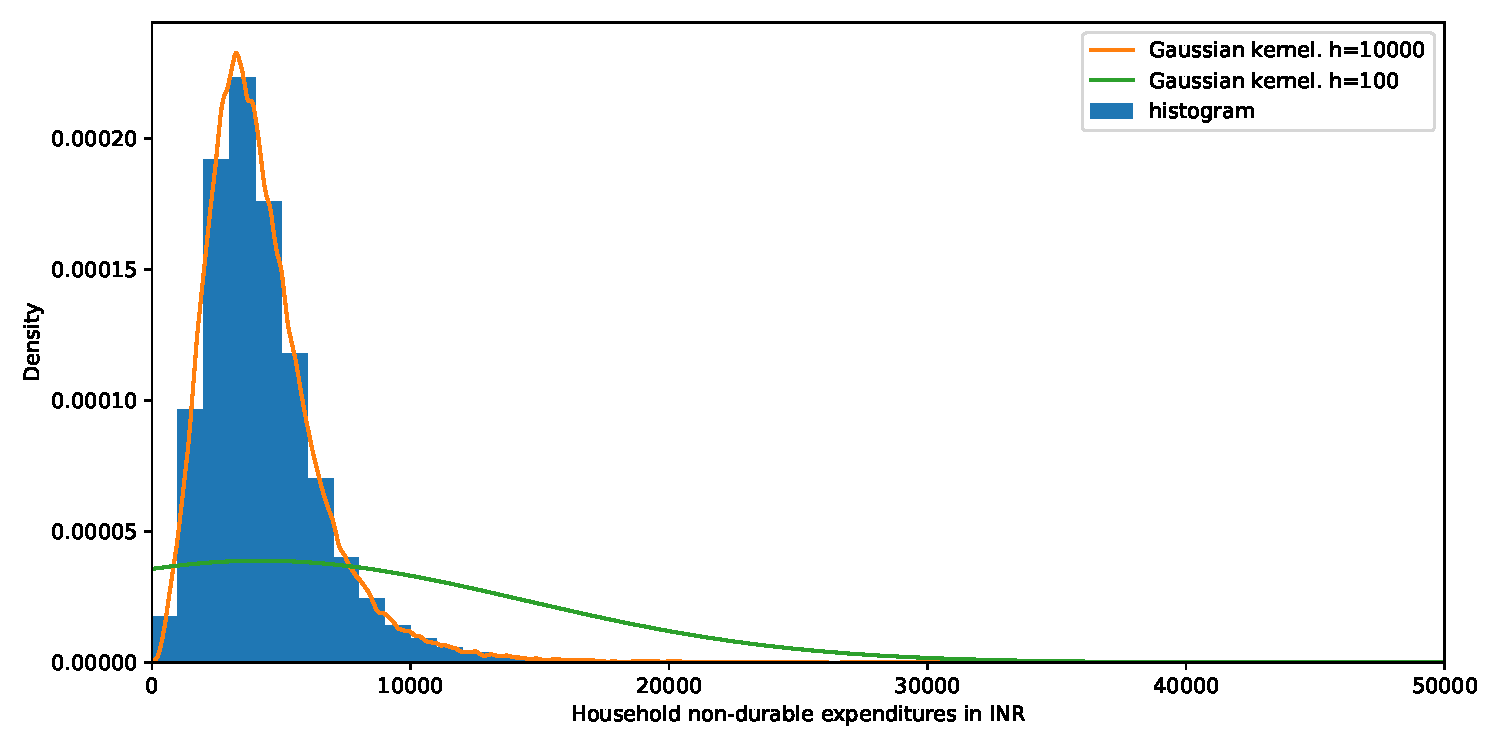
\includegraphics[width=.8\textwidth]{../Output/fig_kernel_trials_gauss_kde.pdf}\caption{Kernel density estimation using a gaussian kernel with different bandwidth sizes.}\label{fig:e7_1}
\end{figure}

\begin{figure}[!h]
    \centering 
    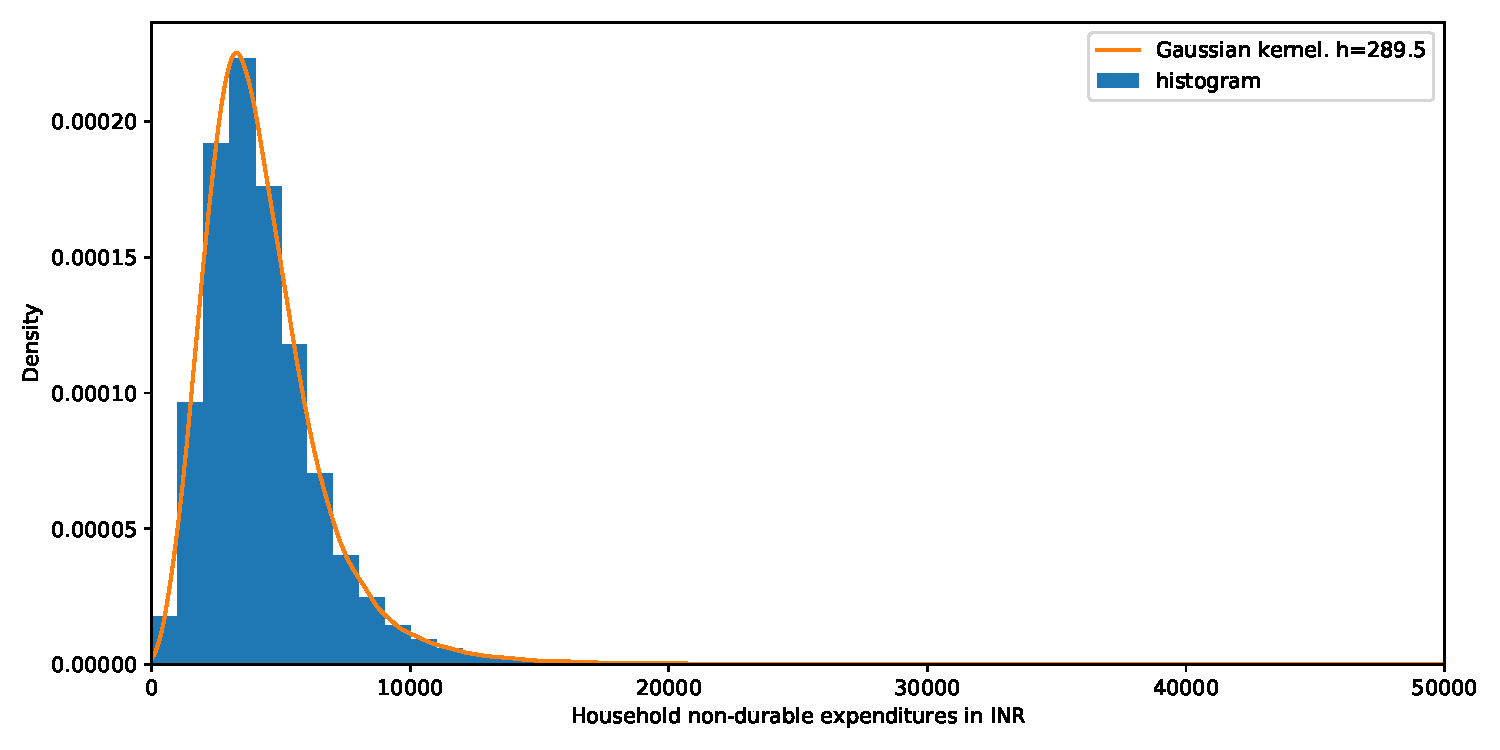
\includegraphics[width=.8\textwidth]{../Output/fig_silverman_gauss_kde.pdf}\caption{Kernel density estimation using a gaussian kernel with the bandwidth size set to Silverman's rule.}\label{fig:e7_2}
\end{figure}




\subsection*{Part 2}
My favorite kernel and bandwidth is the gaussian kernel with the Silverman bandwidth. For the transformation, we want to transform the variable $x$ into $y = g(x) =\log(x)$. Note that $supp(x) = [0, \infty]$, but $supp(g(x)) = R$. Also note that $g^{-1}(y) = e^y$ and $\frac{\partial g^{-1}(y)}{\partial y} = e^y$. So from the inverse Jacobian rule:

\[f_Y(y) = f_X(g^{-1}(y))|\frac{\partial g^{-1}(y)}{\partial y} | = f_X(e^y)e^y \;\; y \in R\]

\noindent Replacing $f_X(\cdot)$ with $\hat{f}^h(x)$ and setting $h$ to be the Silverman bandwidth, we can generate kernel density. Figure \ref{fig:e7_3} plots the transformed density, it is the orange solid line. 

\subsection*{Part 3}
Choosing the gaussian kernel and the Silverman's bandwidth on the logged data, we generated the KDE and plotted it in red dots in Figure \ref{fig:e7_3}. We can see that both approaches provide an almost identical KDE distribution.


\begin{figure}[!h]
    \centering 
    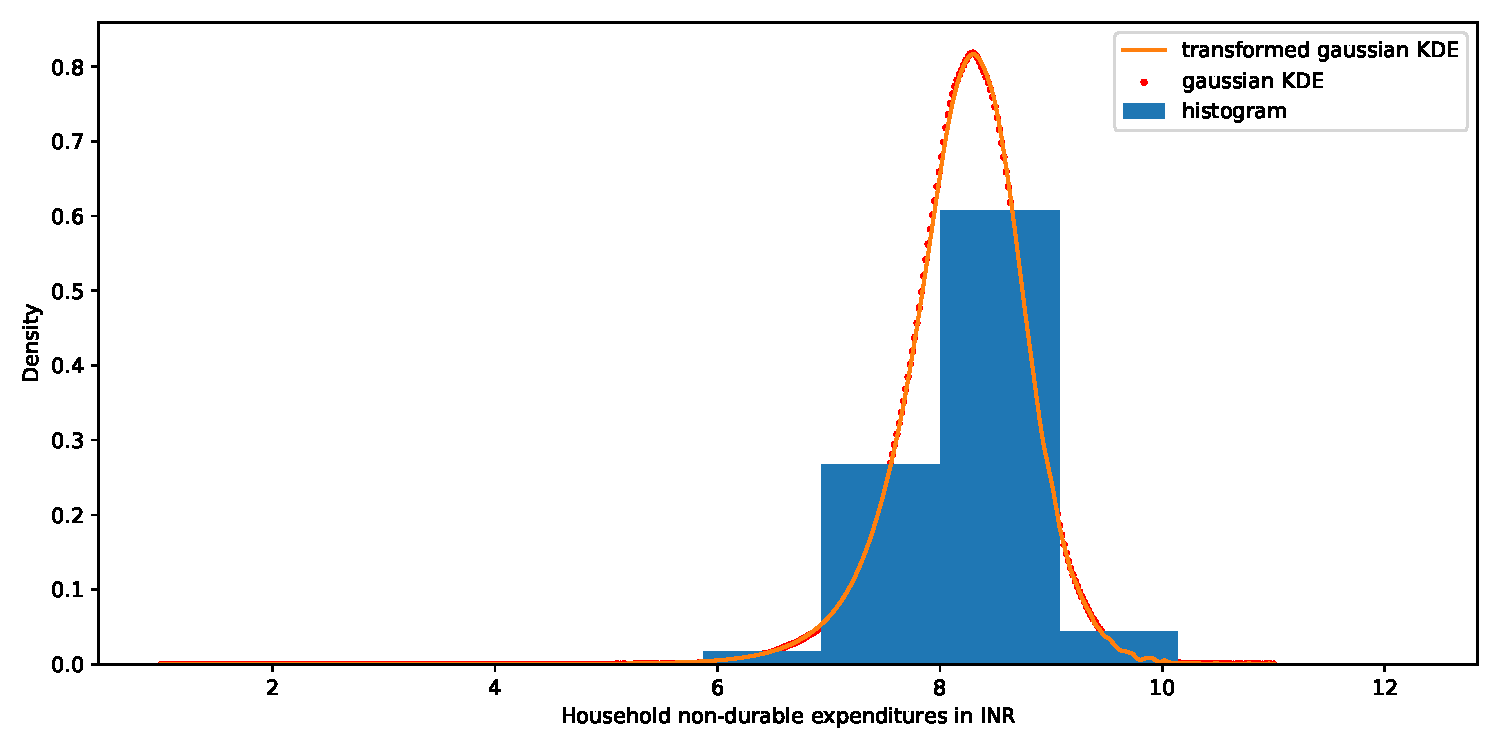
\includegraphics[width=.8\textwidth]{../Output/fig_kernel_transformed_gauss_kde.pdf}\caption{Kernel density estimation using a gaussian kernel. The variable is logged household expenditures. The two estimates are for the transformed and the directly estimated KDE.}\label{fig:e7_3}
\end{figure}

\section*{8. ``Plug-In'' Kernel Bias Estimator}
In class we derived the bias of the kernel density estimator to be :
\[E[\hat{f}(x)] - f(x) = \int K(u) (f(x+hu))du - f(x) =  \int K(u) (f(x+hu)-f(x))du\]

TODO: Ask about. Not sure...

\end{document}
